\label{sec:aggregating}

[[TODO: Updated section to read]]

\begin{definition}
  An algorithm for the \kgs is \emph{$k$-admissible} if in any instance, for all reachable goals $t_i$, the first path found to $t_i$ is optimal.
  An algorithm for the \kgs is \emph{$1$-admissible} if in any instance, there exists a goal $t_i$ such that the first path found to $t_i$ is optimal.
\end{definition}
\abda{check 1-admissible definition in case some goals are not reachable}

%In \astar{} for a single goal, states are prioritized in \open according to the $f=g+h$ value of a state. In contrast, a state in \kastar{} has a vector of $k$ heuristic values $\vect{h}(n)$ and consequently a vector of $f$ values $\vect{f}$(n) that contains one $f$ value per goal. Therefore, \kastar{} requires a state evaluation function that aggregates these $f$ values in some way. In Algorithm~\ref{alg:k-goal-bfs} this is encapsulated in the {\tt ComputeF} function. We refer to the value ($F$) returned by this function as the state's $F$ value, and consider the following two options for computing it.
We consider the following two options for computing the $F$ value of a state:  
\begin{align}
  \text{\minf} =& g(n) + \min_{i\in [1,k]}h_i(n) \\
  \text{\maxf} =& g(n) + \max_{i\in [1,k]}h_i(n)
\end{align}
\kastar that uses \minf as the state evaluation function is referred to hereinafter as \kastarmin, and similarly \kastar that uses \maxf is referred to as \kastarmax. [[AF: If this was not already defined earlier then put this earlier. No need to re-define]]
Before analyzing the theoretical properties of \kastarmin and \kastarmax, we provide the following invariant which holds in \kastar regardless of how the $F$ values are computed.

\begin{lemma}
  \label{lem:simple}
  In every iteration of \kastar, for every active goal $t_i$, there exists a state $n$ in \open on an optimal path to $t_i$, i.e., $g(n) + d(n, t_i) = d(s, t_i)$.
\end{lemma}

Lemma~\ref{lem:simple} can be proven by induction over the iterations of \kastar.
Namely, it trivially holds in the first iteration and continues to hold in subsequent iterations because when a state with $g(\cdot) + d(s,\cdot) = d(s, t_i)$ is expanded then one of its children must also have $g(\cdot) + d(s,\cdot) = d(s, t_i)$.
An equivalent to Lemma~\ref{lem:simple} has been proven for many other best-first search algorithms.

\begin{lemma}[Completeness]
  \label{lem:completeness}
  If a goal state is reachable, then it is eventually expanded by \kastar. [[AF: but not necessarily optimal]
\end{lemma}

\begin{theorem}
  \label{thm:min-f}
  If $h_1,\dots,h_k$ are admissible, then \kastarmin is $k$-admissible.
\end{theorem}
\begin{proof}
  The proof is subsumed by that of Theorem~\ref{thm:admissible} below.
\end{proof}

[[AF: not clear that this is not a repetition. We proved this above. Do we want to claim this again]

\begin{observation}[\kastarmax is not $k$-admissible]
  \label{obs:max-f-inadmissible}
  Running \kastarmax may return a path $\pi_i$ from $s$ to $g_i$ that is not optimal.
\end{observation}

%[[AF: in the theory above you talked about Fmin and here you talk about kastamx. Use kastarmin too.]]\roni{Maybe you looked at an old version?}

To demonstrate Observation~\ref{obs:max-f-inadmissible}, consider the graph in Figure~\ref{fig:max-bad}.
In this example, using \kastarmax results in the following expansion order: $S$, $B$, $t_1$, and $t_2$.
Importantly, state $A$ was not expanded, and so the best path returned for $t_1$ goes through $B$ and costs 3.
A better path to $t_1$ exists, which runs through $A$ and costs only 2.

\begin{figure}
  \centering
  \subfloat{
    \begin{tikzpicture}
      \node[source]  (s)  at (0, 0.7) {$S$};
      \node[other]   (a)  at (3, 1.2) {$A$};
      \node[other]   (b)  at (3, 0.0) {$B$};
      \node[target1] (t1) at (6, 1.2) {$t_1$};
      \node[target2] (t2) at (6, 0.0) {$t_2$};

      \draw[->] (s) -- (a) node[midway] (sa) {\phantom{0}};
      \draw[->] (s) -- (b) node[midway] (sb) {\phantom{0}};
      \draw[->] (a) -- (t1) node[midway] (at1) {\phantom{0}};
      \draw[->] (b) -- (t1) node[midway] (bt1) {\phantom{0}};
      \draw[->] (b) -- (t2) node[midway] (bt2) {\phantom{0}};

      \node[above = -2mm of sa,edgeweight]   {$1$};
      \node[below = -2mm of sb,edgeweight]   {$1$};
      \node[above = -2mm of at1,edgeweight]  {$1$};
      \node[above left = -5mm of bt1,edgeweight]  {$2$};
      \node[below = -2mm of bt2,edgeweight]  {$3$};

      \node[below = 2mm of  s,infobox] {$h=\tuple{0, 0}$};
      \node[above = 2mm of  a,infobox] {$h=\tuple{1, 4}$};
      \node[below = 2mm of  b,infobox] {$h=\tuple{2, 3}$};
      \node[above = 2mm of t1,infobox] {$h=\tuple{0, 0}$};
      \node[below = 2mm of t2,infobox] {$h=\tuple{0, 0}$};
    \end{tikzpicture}
  }
  \hfill
  \subfloat{
    \begin{tabular}[b]{lccc}
      \toprule
      Path & $g$ & $\vect{h}$ & $F$\\
      \midrule
      $SB$    & $1$ & $\tuple{2, 3}$ & $4$ \\
      $SBt_1$ & $3$ & $\tuple{0, 0}$ & $3$ \\
      $SBt_2$ & $4$ & $\tuple{0, 0}$ & $4$ \\
      $SA$    & $1$ & $\tuple{1, 4}$ & $5$ \\
      $SAt_1$ & $2$ & $\tuple{0, 0}$ & $2$ \\
      \bottomrule
    \end{tabular}
  }
  \caption{An example of where using \kastarmax is not $k$-admissible because it returns a non-optimal solution.
    Using \kastarmax results in the following expansion order: $S$, $B$, $t_1$.
    Thus, when $t_1$ is expanded, the best path known to it costs 3, while a better path to $t_1$ goes through $A$ and costs only 2.}
  \label{fig:max-bad}
\end{figure}

Note that the heuristic function $h_2$ in Figure~\ref{fig:max-bad} is inconsistent (Definition~\ref{def:consistent}).
Indeed, we have $h_2(A) = 4 > 0 + 1 = h_2(t_1) + d(A, t_1)$.
On the other hand, when the heuristics used are consistent then \kastarmax is guaranteed to only return optimal paths:
% using \maxf{} is possible [[AF: admissible?]], [[AF: I would only use one term KASTARMAX and never use FMAX. Why do you need both. Your call.]]due to the following result.

\begin{theorem}
  \label{thm:max-f}
  If $h_1,\dots,h_k$ are consistent, then \kastarmax is $k$-admissible.
\end{theorem}
\begin{proof}
  The proof is subsumed by that of Theorem~\ref{thm:consistent} below.
\end{proof}

[[AF: again, there is repetitions of work, I think. Say everything only once]]



%[[AF: I do not like the term maxf and do not like that you say that it is admissible without exactly defining what you mean. Can you omit this and only talk on kastarmax]]\roni{Fixed}. [[ARIEL UP TO HERE]]

[[AF: maybe we just talk on the general case first and then mention that max and min are special cases?]]
\subsection{General Heuristic Aggregation Functions}
The operators $\min$ and $\max$ are two ways to aggregate the heuristic values of a given node, but \kastar can also be implemented with other aggregation functions, functions that accept a vector of $k$ values and output a single value.
\begin{definition}
  Let $k$ be a fixed positive integer.
  A \emph{heuristic aggregation function} is a function $\Phi: \nonnegreals^k \rightarrow \nonnegreals$ such that $\Phi(\vect{0}) = 0$, where $\vect{0}$ is the $k$-dimensional zero vector.
\end{definition}
\kastar can use such a function to computes the $F$ value of a node $n$, as $F(n) = g(n) + \Phi(\vect{h}(n))$, where $\vect{h}(n)$ is the vector $\tuple{h_1(n), h_2(n), \dots, h_k(n)}$.
We denote the resulting algorithm as \kastarphi.
%Such a heuristic aggregation function accepts a vector of $k$ heuristic values of a node  and outputs a single value, which is then used by \kastar to compute node's $F$ value.  Formally,

In the rest of this section, we examine under which assumptions on $\Phi$ and on the heuristics $\vect{h}$ we can obtain optimality guarantees on \kastarphi.
As we shall see, there is a tradeoff between the two types of assumptions.
Making stronger assumptions on the heuristics leads to optimality for a larger range of aggregation functions. [[AF: not sure what the sentence means: it means optimallity]][[AS: Better now?]

\subsection{Arbitrary Heuristics}
%\abda{$\Phi$ needs to be constant $0$.}

\begin{definition}
  \label{def:ucs}
  \emph{Uniform Cost Search (UCS)} is the \kastarvar{0} algorithm where the heuristic aggregation function is the constant 0 function which maps any vector to value 0.
\end{definition}

UCS coincides with Dijkstra's algorithm~\cite{DIJ59,SoCS2011Felner}, a best-first search without a heuristic which prioritizes nodes based on their $g$ values alone.
As a result, UCS finds the optimal path to every reachable state, including every reachable goal---it is $k$-admissible.

\begin{theorem}
  \label{thm:arbitrary}
  For any \kgs and for any tuple of heuristics, UCS is $k$-admissible.
\end{theorem}

UCS does not use any heuristic information and is guaranteed to find the optimal path for each goal.
On the other hand, we can show that UCS is the only \kastar instantiation that is $k$-admissible with arbitrary heuristics.

\begin{theorem}
  \label{thm:arbitrary-dual}
  If a heuristic aggregation function $\Phi$ is not the constant 0, then there exists a \kgs and a tuple of arbitrary heuristics such that \kastarphi is not $k$-admissible.
\end{theorem}
\begin{proof}
  $\Phi$ is not the constant function 0, so there exists a vector $\vect{v}$, such that $\Phi(\vect{v}) > 0$,
  Let $\vect{w} = \vect{0}$, $i = 1$, and $\delta$ such that $\Phi(\vect{v}) > \delta > 0$.
  Note that $w_i = 0$ and that $\Phi(\vect{v}) > \Phi(\vect{w}) + \delta = \delta$ and consider the counter-example in Figure~\ref{fig:kstarphi-bad}. [[AF: not clear what are the different variables? nodes? just variables? Also, I think the text in the caption should be placed in the main text]][[AF: I suggest to move all the vector from bold to a letter with a bar above or bellow]]
\begin{figure}
  \centering
  \subfloat{
  \begin{tikzpicture}
    \node[source] (s) at (0, 2) {$S$};
    \node[other]  (a) at (4, 2) {$A$};
    \node[target1] (b) at (4, 0) {$B$};
    \node[target2] (c) at (0, 0) {$C$};

    \draw[->] (s) -- (a) node[midway] (sa) {\phantom{0}};
    \draw[->] (s) -- (b) node[midway] (sb) {\phantom{0}};
    \draw[->] (s) -- (c) node[midway] (sc) {\phantom{0}};
    \draw[->] (a) -- (b) node[midway] (ab) {\phantom{0}};

    \node[above = -2mm of sa,edgeweight] {$\epsilon$};
    \node[below left = -5mm of sb,edgeweight] {$\delta + 2\epsilon$};
    \node[left  = -2mm of sc,edgeweight] {$\Phi(\vect{v})$};
    \node[right = -2mm of ab,edgeweight] {$\delta$};

    \node[left  = 2mm of  s,infobox] {$\vect{h}=\vect{0}$};
    \node[right = 2mm of  a,infobox] {$\vect{h}=\vect{v}$};
    \node[right = 2mm of  b,infobox] {$\vect{h}=\vect{w}$};
    \node[left  = 2mm of  c,infobox] {$\vect{h}=\vect{0}$};
  \end{tikzpicture}
  } \hfill
  \subfloat{
    \begin{tabular}[b]{lccc}
      \toprule
      Path & $g$ & $H$ & $F$\\
      \midrule
      $SB$ & $\delta + 2\epsilon$ & $\Phi(\vect{w})$ & $\Phi(\vect{v}) - \epsilon$ \\
      $SC$ & $\Phi(\vect{v})$ & $0$ & $\Phi(\vect{v})$\\
      $SA$ & $\epsilon$ & $\Phi(\vect{v})$ & $\Phi(\vect{v}) + \epsilon$ \\
      $SAB$ & $\delta + \epsilon$ & $\Phi(\vect{w})$ & $\Phi(\vect{v}) - 2\epsilon$ \\
      \bottomrule
    \end{tabular}
  }
  \caption{Generic counter-example for \kastarphi.
    Let $\vect{v}$, $\vect{w}$, $i$, and $\delta$ such that $w_i = 0$, $\delta > 0$, and $\Phi(\vect{v}) > \Phi(\vect{w}) + \delta$.
    Define $\epsilon = \frac{\Phi(v) - \Phi(\vect{w}) - \delta}{3} > 0$.
    We use the weighted graph displayed above left where $S$ is the start state, $B$ is the $i$\textsuperscript{th} goal and $C$ is the $j$\textsuperscript{th} goal for $j \neq i$.
     As can be seen from the table above right, the search expands $S$, $B$, $C$, then stops.
     The optimal path to $B$ is $SAB$, but \kastarphi returns the suboptimal path $SB$.}
  \label{fig:kstarphi-bad}
\end{figure}
\end{proof}


\subsection{Admissible Heuristics}
\begin{definition}
  A heuristic aggregation function $\Phi$ is \emph{\axiomadm} iff for every vector $\vect{v}$, we have $\Phi(\vect{v}) \leq \min \vect{v}$.
\end{definition}
[[AF: adm-compat???]]
\begin{observation}
  $\Phi = 0$ and $\Phi=\min$ are \axiomadm.
\end{observation}

\begin{theorem}
  \label{thm:admissible}
  Let $\Phi$ be a \axiomadm heuristic aggregation function.
  For any \kgs and for any tuple of admissible heuristics $\vect{h}$, \kastarphi is $k$-admissible.
\end{theorem}
\begin{proof}
  Assume that \kastarphi chooses to expand a goal node $t$ (i.e., $t=t_i\in\{t_1,\ldots t_k\}$).
  Applying Lemma~\ref{lem:simple} to $t_i$, we obtain $n\in \open$ such that $g(n) + d(n, t_i) = d(s, t_i)$.
  Since $t$ is expanded before $n$, we have $g(t) + \Phi(\vect{h}(t)) = F(t) \leq F(n) = g(n) + \Phi(\vect{h}(n))$.

  \begin{align}
    h_i(n) & \leq d(n,t_i) & \text{($h_i$ is admissible)}\\
    \Phi(\vect{h}(n)) \leq \min_j h_j(n) & \leq d(n,t_i) & \text{($\Phi$ is \axiomadm)}\\
    g(n) + \Phi(\vect{h}(n)) & \leq g(n) + d(n, t_i) = d(s, t_i) & \text{($n$ is chosen via Lemma~\ref{lem:simple})}\\
    F(t) \leq F(n) & \leq d(s, t_i) & \text{($t$ is expanded before $n$)}\\
    g(t) + \Phi(\vect{h}(t)) & \leq d(s, t_i) & \text{(by definition of $F$)}\\
    g(t) & \leq d(s, t_i) & \text{($\Phi$ is non-negative)}\\
    d(s, t_i) \leq g(t) & \leq d(s, t_i) & \text{(by definition of $d$)}
%    \label{eq:admissible}
  \end{align}
  Therefore, when we expand a goal its $g$ value is equal to $d(s,t_i)$ as required.
\end{proof}

Theorem~\ref{thm:admissible} shows that being \axiomadm is a sufficient condition for optimality of \kastarphi with admissible heuristics.
Our next result shows that it is a necessary condition.

\begin{theorem}
  \label{thm:admissible-dual}
  If a heuristic aggregation function $\Phi$ is not \axiomadm, then there exists a \kgs and a tuple of admissible heuristics such that \kastarphi is not $k$-admissible.
\end{theorem}
\begin{proof}
  Let $\vect{v}$ such that $\Phi(\vect{v}) > \min \vect{v}$.
  Let $\vect{w} = \vect{0}$, $i = \argmin \vect{v}$, and $\delta$ such that $\Phi(\vect{v}) > \delta > \min \vect{v} = v_i$.
  Note that $\Phi(\vect{v}) > \Phi(\vect{w}) + \delta$ and consider the counter-example in Figure~\ref{fig:kstarphi-bad}.

  To conclude the proof, it remains to observe that the heuristics involved are admissible.
  This is indeed the case because we have $h_i(A) \leq \min \vect{v} \leq \delta = d(A, B)$ and therefore $h_i(A) \leq d(A, B)$.
\end{proof}

[[AF: doesn't this mean that MIN is the only reasonable function that is k-admissible? Anything smaller than min is not reasonable in my option. It is like cutting a heuristic down]

\begin{theorem}
  \label{the:kastarmin-surely}
  For any \kgs and for any tuple of admissible heuristics $\vect{h}$, \kastarmin expands all the surely expanded states.
\end{theorem}
\begin{proof}
%  Consider the \open and \closed lists when the last goal is expanded.
  By negation, let $n$ be a state that is surely expanded w.r.t. $t_i$ but is not expanded by \kastarmin.
  That is, $n$ is reachable from $s$ by a path of states with $f_i$  values lower than $d(s, t_i)$ and $f_i(n) < d(s, t_i)$.
  Since we are using $\Phi = \min$, the $F$ values of the states along this path must also be lower than $d(s, t_i)$.
  As all edges in the underlying graph have non-negative cost, $h_i(t_i) = 0$ and therefore $F(t_i) = d(s, t_i)$.
  Hence, the minimal $F$ value in \open is $d(s, t_i)$ when $t_i$ is expanded.
  Thus, all the states along the path to $n$ and $n$ itself must have already been expanded, as all of them have $f_i$ values smaller than $d(s, t_i)$ and thus also have $F$ values smaller than $d(s, t_i) = F(t_i)$.
\end{proof}
\abda{Probably more than just \kastarmin.}


[[AF: probably all the adm-compact functions??]

\subsection{Consistent Heuristics}

\begin{definition}
  A heuristic aggregation function $\Phi$ is \emph{\axiomcons} iff for every vectors $\vect{v}$ and $\vect{w}$, we have $\exists i, w_i = 0 \implies \Phi(\vect{v}) - \Phi(\vect{w}) \leq \max (\vect{v}-\vect{w})$.
\end{definition}

[[AF: not clear what is $w_i$? ]
%\abda{Alternative names: \emph{metric}, \emph{weak contraction}. See \url{https://en.wikipedia.org/wiki/Metric_map} for inspiration.}
% Similar to \cite{Denardo1967}

\begin{theorem}
  \label{thm:consistent}
  Let $\Phi$ be a \axiomcons heuristic aggregation function.
  For any \kgs and for any tuple of consistent heuristics $\vect{h}$, \kastarphi is $k$-admissible.
\end{theorem}
\begin{proof}
  Assume that \kastar chooses to expand a goal node $t$ (i.e., $t = t_i \in \{t_1, \ldots t_k\}$) via a path $p$.
  Applying Lemma~\ref{lem:simple} to $t_i$, we obtain $n\in \open$ such that $g(n) + d(n, t_i) = d(s, t_i)$.
  Since $t$ is expanded before $n$, we have $g(t) + \Phi(\vect{h}(t)) = F(t) \leq F(n) = g(n) + \Phi(\vect{h}(n))$.

  \begin{align}
    h_j(n)                             & \leq d(n, t_i) + h_j(t_i) & \text{(for all $j$, $h_j$ is consistent)}\\
    h_j(n) - h_j(t_i)                  & \leq d(n, t_i)              & \text{(for all $j$)}\\
    \max (\vect{h}(n) - \vect{h}(t_i)) & \leq d(n, t_i)              & \text{}\\
%    \Phi(\vect{h}(n)) - \Phi(\vect{h}(t_i)) & \leq d(n, t_i) & \text{($\Phi$ is \axiomcons and $h_i(t_i) = 0$)}\\
    \Phi(\vect{h}(n))                  & \leq d(n, t_i) + \Phi(\vect{h}(t_i)) & \text{($\Phi$ is \axiomcons and $h_i(t_i) = 0$)}\\
    g(n) + \Phi(\vect{h}(n))           & \leq d(s, t_i) + \Phi(\vect{h}(t_i)) & \text{($n$ is chosen via Lemma~\ref{lem:simple})}\\
    F(t) \leq F(n)                     & \leq d(s, t_i) + \Phi(\vect{h}(t_i)) & \text{($t$ is expanded before $n$)}\\
    g(t) + \Phi(\vect{h}(t))           & \leq d(s, t_i) + \Phi(\vect{h}(t_i)) & \text{(by definition of $F$)}\\
    d(s, t_i) \leq g(t)                & \leq d(s, t_i) & \text{(by definition of $d$)}
    \label{eq:consistent}
  \end{align}
  Therefore, when we expand a goal its $g$ value is equal to $d(s, t_i)$ as required.
\end{proof}

Theorem~\ref{thm:consistent} shows that being \axiomcons is a sufficient condition for optimality of \kastarphi with consistent heuristics.
Our next result shows that it is a necessary condition.

\begin{theorem}
  \label{thm:consistent-dual}
  If a heuristic aggregation function $\Phi$ is not \axiomcons, then there exists a \kgs and a tuple of consistent heuristics such that \kastarphi is not $k$-admissible.
\end{theorem}
\begin{proof}
  $\Phi$ is not \axiomcons, so there exists vectors $\vect{v}$, $\vect{w}$, and an index $i$ such that $w_i = 0$ and $\Phi(\vect{v}) - \Phi(\vect{w}) > \max (\vect{v} - \vect{w})$.
  Let $\delta$ such that $\Phi(\vect{v}) - \Phi(\vect{w}) > \delta > \max (\vect{v} - \vect{w})$.
  Recall that $v_i \geq 0$, so $\max (\vect{v} - \vect{w}) \geq v_i - w_i \geq 0$, therefore $\delta > 0$.
  Consider the counter-example in Figure~\ref{fig:kstarphi-bad}.

  To conclude the proof, it remains to observe that the heuristics involved are consistent.
  This is indeed the case because for all $j$, we have $h_j(A) - h_j(B) = v_j - w_j \leq \max (\vect{v} - \vect{w}) < \delta = d(A, B)$ and therefore $h_j(A) \leq d(A, B) + h_j(B)$.
\end{proof}

Theorem~\ref{thm:consistent} opens the opportunity to run \kastar for a larger range of heuristic aggregation functions than Theorem~\ref{thm:admissible}, provided the heuristic functions are consistent.

\begin{observation}
  Any \axiomadm function is also \axiomcons.
%  In particular $\Phi=\min$ is \axiomcons.
\end{observation}
\begin{proof}
  Let $\Phi$ be an \axiomadm heuristic aggregation function and let $\vect{v}$ and $\vect{w}$ be vectors such that $\exists i, w_i = 0$.
  On the one hand, $\Phi(\vect{v}) - \Phi(\vect{w}) \leq \Phi(\vect{v}) \leq \min \vect{v} \leq v_i$.
  On the other hand, we have $w_i = 0$ so we derive $v_i \leq v_i - w_i \leq \max (\vect{v} - \vect{w})$.
  As result, $\Phi(\vect{v}) - \Phi(\vect{w}) \leq \max (\vect{v} - \vect{w})$, and we conclude that $\Phi$ is \axiomcons.
\end{proof}

Let $\{ v_i \}$ be a collection of terms. [[AF: what does that mean? numbers? Who is i? do you have vi, v2 etc?]][[AF: do you want to start a new definition here?]]
A \emph{subconvex} combination of these terms is a linear combination $\sum_i \alpha_i t_i$ where all coefficients are non-negative, $0 \leq \alpha_i$, and the sum of coefficients is no more than one, $\sum_i \alpha_i \leq 1$.

The $i$th \emph{order statistic} of a vector $\vect{v}$ is the $i$th smallest value of $\vect{v}$ and is denoted $v_{(i)}$. [[AF: why not just call it i'th smallest?]
For instance, if $\vect{v} = \tuple{3, 1, 0, 1}$, then $v_{(1)} = v_3 = 0$, $v_{(2)} = v_{(3)} = v_2 = v_4 = 1$ and $v_{(4)} = v_1 = 3$. [[AF: this is just a permutation along the values]

[[AF: jumped further. I am happy to sit down with whoever wrote this to further polish the text]

The \axiomcons axiom is not only as general as \axiomadm, but it also allows for aggregation functions not covered by the previous assumption:
\begin{theorem}
  \label{thm:subconvex}
  Subconvex combinations of the components and the order statistics give rise to \axiomcons heuristic aggregation functions.
\end{theorem}
\begin{proof}
  Consider $2k$ non-negative coefficients $\alpha_i$ such that $\sum_{1 \leq i \leq 2k} \alpha_i \leq 1$.
  Then, we will show that $\Phi$ defined as $\Phi(\vect{v}) = \sum_{1 \leq i \leq k} \alpha_i v_i + \alpha_{k+i} v_{(i)}$ is a heuristic aggregation function.
  For any two vectors $\vect{v}$ and $\vect{w}$, we have $\Phi(\vect{v}) - \Phi(\vect{w}) = \sum_{1 \leq i \leq k} \alpha_i (v_i - w_i) + \alpha_{(i+k)} (v_{(i)} - w_{(i)})$.
  On the one hand, $v_i - w_i \leq \max (\vect{v} - \vect{w})$ is direct, on the other hand, $v_{(i)} - w_{(i)} \leq \max (\vect{v} - \vect{w})$ can be established with a little bit more effort:

  Indeed, for $1 \leq i \leq k$, define $V_i = \{j, v_j < v_{(i)} \}$ and $W_i = \{j, w_j < w_{(i)} \}$ and observe that $|V_i| \leq i - 1$ and $|W_i| \leq k - i$ by definition of the order statistics.
  It follows that $|V_i \cup W_i| \leq k - 1$.
  From a counting argument, obtain an integer $1 \leq l_i \leq k$ such that $l_i \notin V_i \cup W_i$.
  By construction of $V_i$ and $W_i$, deduce that $v_{(i)} \leq v_{l_i}$ and that $w_{l_i} \leq w_{(i)}$ and conclude that $v_{(i)} - w_{(i)} \leq v_{l_i} - w_{l_i} \leq \max (\vect{v} - \vect{w})$.

  As a result, we have $\Phi(\vect{v}) - \Phi(\vect{w}) \leq \sum_{1 \leq i \leq 2k} \alpha_i \max(\vect{v} - \vect{w})$ because for all $i$, $\alpha_i$ is non-negative.
  Therefore, $\Phi(\vect{v}) - \Phi(\vect{w}) \leq \max(\vect{v} - \vect{w}) \sum_i \alpha_i \leq \max(\vect{v} - \vect{w})$, thus showing that $\Phi$ is \axiomcons.
\end{proof}

\begin{corollary}
  Using any of the \emph{mean}, the \emph{maximum}, the \emph{minimum}, the \emph{$i$th projection}, for $1 \leq i \leq k$, or the \emph{median} of the values in $\vect{v}$ gives a \axiomcons heuristic aggregation function.
\end{corollary}
\begin{proof}
  All these quantities can be expressed as subconvex combinations of the components and the order statistics, so they are all \axiomcons:
  The $i$th projection is $\Phi(\vect{v}) = v_i$; the \emph{mean} is $\Phi(\vect{v}) = \frac{v_1 + \dots + v_k}{k}$; the \emph{maximum} is $\Phi(\vect{v})= v_{(k)}$; the \emph{minimum} is $\Phi(\vect{v}) = v_{(1)}$; and the \emph{median} is $\Phi(\vect{v}) = \frac{1}{2}(v_{(\frac{k}{2})} + v_{(\frac{k+1}{2})})$.
\end{proof}

It is easy to show that for $2 \leq k$, none of these heuristic aggregation function is \axiomadm, except for the \emph{minimum}.
Thus, Theorem~\ref{thm:consistent} does indeed extend the range of functions for which we can obtain guarantees to other natural aggregation methods.

\begin{observation}
  The following heuristic aggregation functions do not satisfy \axiomcons.
  The \emph{sum} aggregation, $\Phi(\vect{v}) = \sum_i v_i$ is not \axiomcons as soon as there are two goals or more.
  More generally, combinations of the components that are not subconvex do \emph{not} give rise to \axiomcons heuristic aggregation functions.
\end{observation}
\begin{proof}
  Consider non-negative coefficients $\alpha_i$ such that $\sum_i \alpha_i > 1$.
  Then, $\Phi$ defined as $\Phi(\vect{v}) = \sum_i \alpha_i v_i$ is a heuristic aggregation function.
  However, taking for instance $\vect{v} = \vect{1}$ and $\vect{w} = \vect{0}$, we have $\vect{v} - \vect{w} = \sum_i \alpha_i (1 - 0) = \sum_i \alpha_i > 1 = \max (\vect{v} - \vect{w})$.
  Therefore $\Phi$ is not \axiomcons.
  In particular, the sum aggregation function is not \axiomcons.
\end{proof}

\begin{observation}
  The \emph{range statistic}, $\Phi(\vect{v}) = v_{(k)} - v_{(1)}$, is \axiomcons.
  For $k \geq 3$, the ``almost-range'' statistic defined as $\Phi(\vect{v}) = v_{(k)} - v_{(2)}$ is not \axiomcons.
\end{observation}
\begin{proof}
\abda{blabla}
\end{proof}

%\subsection{blabla}

\begin{theorem}
  \label{the:kastarmin-surplus}
  For any \kgs and for any tuple of consistent heuristics $\vect{h}$, \kastarmin never expands a surplus state.
\end{theorem}
\begin{proof}
  Let $n$ be a node expanded by \kastarmin.
  Let $i$ be such that $h_i(n) = \min h_i(n)$.
  Applying Lemma~\ref{lem:simple} to $t_i$, we obtain $n_i \in \open$ such that $g(n_i) + d(n_i, t_i) = d(s, t_i)$.
  For any node $p$ on the path from $s$ to $n$, we have the following derivation.
  \begin{align}
    h_i(p)        & \leq d(p, n) + h_i(n)         & \text{($h_i$ is consistent)}\\
    h_i(p)        & \leq d(p, n) + \Phi(\vect{h}(n))         & \text{(from the choice of $i$)}\\
    g(p) + h_i(p) & \leq g(p) + d(p, n) + \Phi(\vect{h}(n)) & \text{}\\
    g(p) + h_i(p) & \leq g(n) + \Phi(\vect{h}(n))          & \text{Lemma blabla}\\
    g(p) + h_i(p) & \leq F(n)         & \text{(by definition of $F$)}\\
    g(p) + h_i(p) & \leq F(n_i) = g(n_i) + \Phi(\vect{h}(n_i))      & \text{($n$ is expanded)}\\
    g(p) + h_i(p) & \leq g(n_i) + h_i(n_i) & \text{(by definition of $\Phi$)}\\
    g(p) + h_i(p) & \leq g(n_i) + d(n_i, t_i) & \text{($h_i$ is admissible)}\\
    g(p) + h_i(p) & \leq d(s, t_i) & \text{($n_i$ is chosen via Lemma~\ref{lem:simple})}
    \label{eq:nosurplus}
  \end{align}
  Thus, $n$ is not surplus for the SPP $\Pi_i$.
  Therefore, $n$ is not surplus for the \kgs.
\end{proof}

Note that our assumption that $h_1, \ldots h_k$ are consistent is necessary for the proof of Theorem~\ref{the:kastarmin-surplus}.
With an admissible but inconsistent heuristic, \kastarmin may, in fact, expand surplus states.
Figure~\ref{fig:inconsistent} shows a \kgs problem with $k = 2$ where this occurs.
\kastarmin will expand all states in the figure, while $B$ is surplus for both goals.

\begin{figure}
%  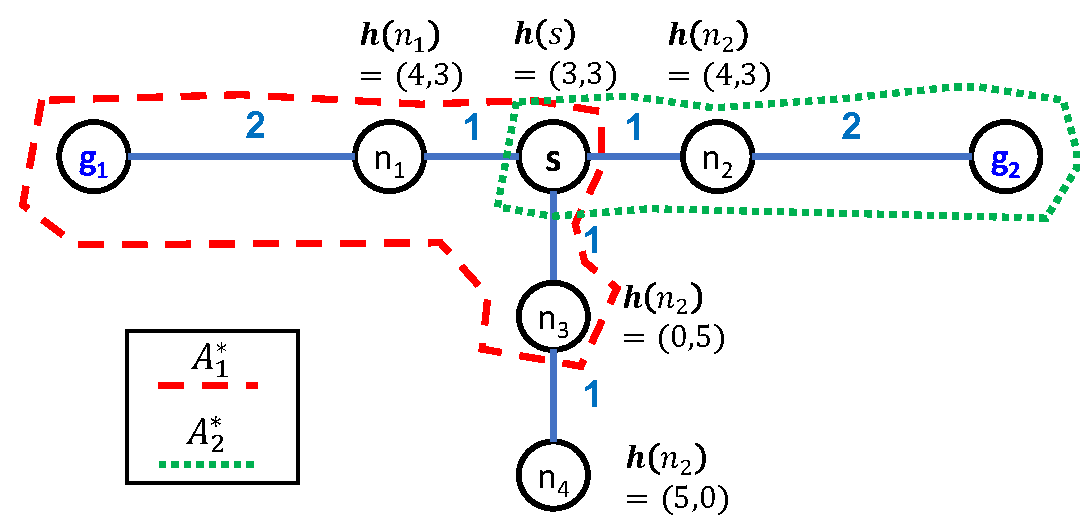
\includegraphics[width=\columnwidth]{inconsistent_cropped.pdf}
  \subfloat{
    \begin{tikzpicture}
    \node[source]  (s)  at (0, 2) {$S$};
    \node[other]   (a)  at (2, 0) {$A$};
    \node[other]   (b)  at (4, 0) {$B$};
    \node[target1] (t1) at (0, 0) {$t_1$};
    \node[target2] (t2) at (3, 2) {$t_2$};

    \draw[->] (s) -- (a)  node[midway] (sa) {\phantom{0}};
    \draw[->] (a) -- (b)  node[midway] (ab) {\phantom{0}};
    \draw[->] (s) -- (t1) node[midway] (st1) {\phantom{0}};
    \draw[->] (s) -- (t2) node[midway] (st2) {\phantom{0}};

    \node[above right = -5mm of sa,edgeweight] {$1$};
    \node[above = -2mm of ab,edgeweight] {$1$};
    \node[left  = -2mm of st1,edgeweight] {$3$};
    \node[above = -2mm of st2,edgeweight] {$3$};

    \node[above = 1mm of  s,infobox] {$\vect{h}=\vect{0}$};
    \node[below = 0mm of  a,infobox] {$\vect{h}=\tuple{0, 5}$};
    \node[below = 0mm of  b,infobox] {$\vect{h}=\tuple{5, 0}$};
    \node[below = 1mm of  t1,infobox] {$\vect{h}=\tuple{0, 5}$};
    \node[above = 0mm of  t2,infobox] {$\vect{h}=\tuple{5, 0}$};
  \end{tikzpicture}
  } \hfill
  \subfloat{
    \begin{tabular}[b]{l*8{c}}
      \toprule
      \multirow{2}{*}{Path} &     & \multicolumn{2}{c}{\astari{1}} & \multicolumn{2}{c}{\astari{2}} & \multicolumn{3}{c}{\kastarmin} \\
      \cmidrule(r){3-4} \cmidrule(lr){5-6} \cmidrule(l){7-9}
              & $g$ & $f$ & S  & $f$ & S  & $H$ & $F$ & S \\
      \midrule
      $S$    & $0$ & $0$ & \xmark & $0$ & \cmark & $0$ & $0$ & \xmark \\
      $St_1$ & $3$ & $3$ & \xmark & $8$ & \cmark & $0$ & $3$ & \xmark \\
      $St_2$ & $3$ & $8$ & \cmark & $3$ & \xmark & $0$ & $3$ & \xmark \\
      $SA$   & $1$ & $1$ & \xmark & $6$ & \cmark & $0$ & $1$ & \xmark \\
      $SAB$  & $2$ & $7$ & \cmark & $2$ & \cmark & $0$ & $2$ & \cmark \\
      \bottomrule
    \end{tabular}
  }
  \caption{An example where \kastarmin expands a surplus state, $B$.
    The table on the right indicates which nodes are expanded and whether the corresponding state is surplus (S) for \astari{1}, \astari{2}, and \kastarmin.
    This example relies on the inconsistency of the second heuristic: $h_2(A) >  d(A, B) + h_2(B)$.
  }
  \label{fig:inconsistent}
\end{figure}

An equivalent theorem for \kastarmax does not hold.
Indeed, there are cases where \kastarmax expands surplus states.
For example, consider the \kgs problem in Figure~\ref{fig:need-resort}.
State $A$ will be expanded first, having $F_{max}(A) = 7$, followed by $B$ ($F_{max}(B) = 8$), $t_2$ ($F_{max}(t_2) = 12$), and finally $t_1$ ($F_{max}(t_1) = 15$).
However, neither \astari{1} nor \astari{2} will expand $A$.
Moreover, $A$ is surplus w.r.t. both $\Pi_1$ and $\Pi_2$, since the optimal path to $t_1$ and $t_2$ costs 6 and 3, respectively, while $f_1(A) = 7 > 6$ and $f_2(A) = 5 > 3$.


%* NTheorem 2 (subsumes Theorem 2/Corollary 2): If A satisfies NAxiom 2 and if h are consistent, then kA*_A is optimal for all k goals. Proof sketch: see below
